\section{Anwendungsfälle}

\subsection{Use Case Diagram}

\begin{figure}[htb]
 \begin{center}
  \leavevmode
  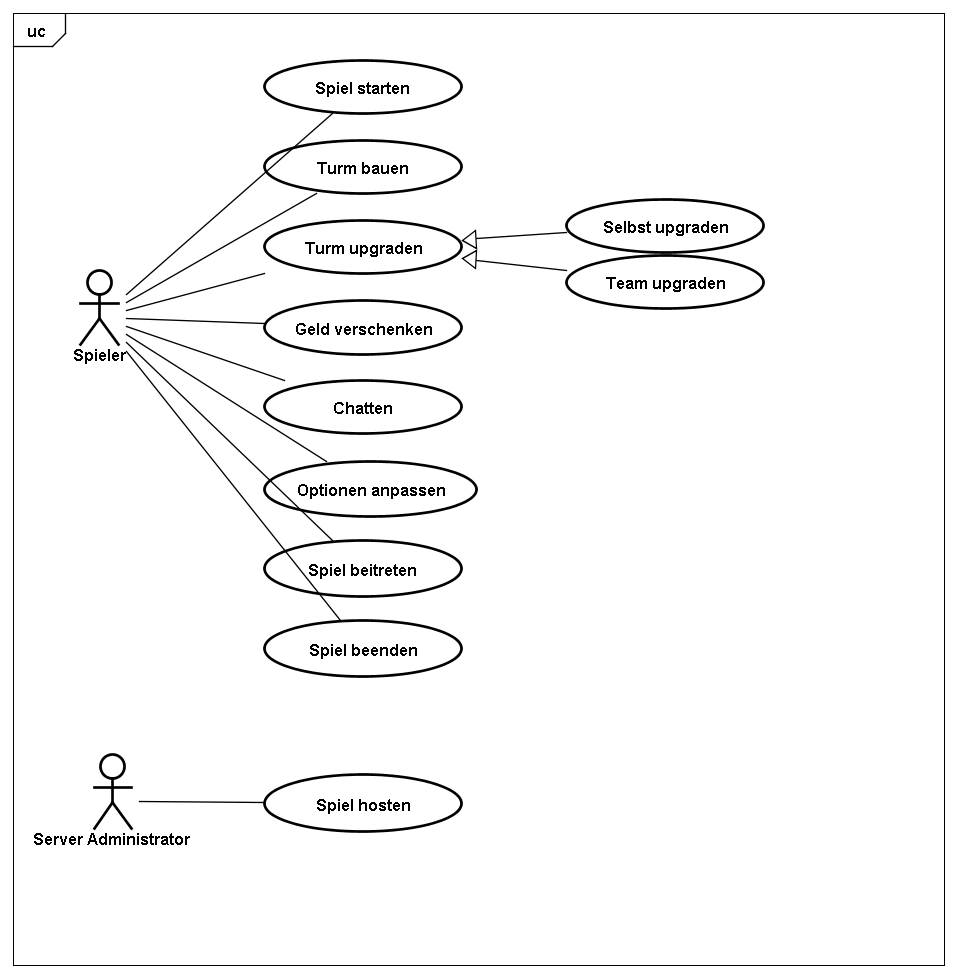
\includegraphics[width=0.95\textwidth]{usecasediagram.png}
 \end{center}
 \caption{Use Case-/Anwendungsfall-Diagram}
 \label{fig:usecasediagram}
\end{figure}

Es existieren zwei Hauptaktoren. Ein Spieler und ein Server Administrator. Total können maximal vier Spieler an einem Spiel teilnehmen. Pro Spiel benötigt es mindestens einen Server Administrator. Der Server Administrator zählt gleichzeitig auch als Spieler. Für ein Einzelspieler Spiel muss braucht es also einen Server Administrator der gleichzeitig auch als Spieler fungiert. Für Multiplayer Spiele können dann jedoch noch bis zu drei zusätzliche Spielern beitreten nebst dem Server Administrator.

Wir haben als Haupt Use Case `Spiel starten' ausgewählt. Als Casual haben wir `Spiel hosten', `\glossary{name={Turm}, description={Eine Einheit, die vom Benutzer gebaut wird und autonom auf Creeps schiesst.}}{Turm} bauen' und `Turm upgraden' ausgewählt. Als Brief stehen somit noch `Spiel beitreten', `Geld verschenken', `Chatten', `Optionen anpassen', `Spiel beenden' und die beiden Upgrade Funktionalitäten `Selbst upgraden' und `Team upgraden' zur Verfügung. Diese beiden Upgrade Funktionalitäten stellen zwei Ausprägungen des `Turm upgraden' dar, da sie unterschiedlich funktionieren, je nach dem ob man einen eigenen Turm oder den Turm eines Kollegen upgraden möchte.

\subsection{Use Case UC1: Spiel starten}

\textbf{Primary Actor:} Spieler

\textbf{Stakeholder and Interests:}

\begin{itemize}
\item Spieler: Möchte so schnell wie möglich ein Spiel starten und keine grosse Verzögerung durch die Authentifizierung
\item Server: Möchte die Verbindungen verwalten
\end{itemize}

\textbf{Precondition:}
\begin{itemize}
\item Der Spieler möchte ein Spiel starten 
\item Es muss ein Server aktiv sein
\end{itemize}


\textbf{Postcondition:}
\begin{itemize}
\item Programm ist offen und eine Verbindung steht
\end{itemize}


\textbf{Main Success Scenario:}

\begin{enumerate}
\item Spieler startet Programm
\item Programmfenster erscheint
\item Spieler gibt, falls nicht gespeichert, Spielername ein 
\item Spieler wählt Einzelspiel oder Multiplayer

\begin{enumerate}
\item Spieler wählt Einzelspiel

\begin{enumerate}
\item Programm startet ein Einzelspiel
\item Programm verwaltet Spiel
\end{enumerate}

\item Spieler wählt Multiplayer
\begin{enumerate}
\item Spieler kann wählen, ob er ein Spiel hosten möchte (UC2) oder einem Spiel beitreten möchte (UC3)
\item Spieler wartet dann in der Lobby, bis genügend andere Spieler anwesend sind
\end{enumerate}

\end{enumerate}

\end{enumerate}


\textbf{Extensions:}
\begin{itemize}
\item Wenn während eines Multiplayer Matches das Programm abstürzt oder die Verbindung verloren geht, soll der Server das erkennen und entsprechend reagieren.
\item Wenn der Spielerhost die Verbindung verliert, bricht das Spiel ab.
\end{itemize}

\textbf{Special Requirements:}

Die Fenstergrösse des Programms soll variabel sein


\textbf{Technology and Data Variations List:}

-


\textbf{Frequency of Occurrence:}

Zu Beginn


\textbf{Open Issues:}

-





\subsection{Use Case UC2: Spiel hosten}

\textbf{Primary Actor:} Server Administrator

Ein Spieler startet einen Spiel-Server auf den sich die Clients einloggen können.

Der Server überprüft den Spielername und verwaltet alle aktiven Verbindungen. Wenn alle Spieler bereit sind, wird das Spiel gestartet.

\glossary{name={Wave}, description={(Welle), besteht aus einer variirenden Anzahl an Creeps, die zusammen auf das Spielfeld tretten}}{Wave}
Der hostende Client übernimmt dann das Wave-Handling und das Creep-Handling.

Wenn eine Verbindung zu einem Spieler verloren geht, informiert er die anderen Spieler.

\glossary{name={Spawn-Point}, description={Sind die Punkte auf der Karte, wo die Creeps auf das Spielfeld tretten}}{Spawn-Point}
Wenn ein Spieler seine Verbindung trennt, entfernt er die Türme des entsprechenden Spielers und auch den zugehörigen Wave-Spawn-Punkt.




\subsection{Use Case U3: Spiel beitreten}
\textit{Brief}

\textbf{Primary Actor:} Spieler

Ein Spieler kann einem Match beitreten. Dies kann er über die Adresse tun.




\subsection{Use Case UC4: Turm bauen}

\textbf{Primary Actor:} Spieler

Das Spielfeld muss zusammengestellt werden. Das Spielfeld besteht aus einer (oder mehreren) Hintergrundgrafik, 
begrenzte Bauflächen, Spawn-Punkte für die Creeps, eine Route für die Creeps, Spielinfozeile und einem Baumenü.

Die Creeps müssen dynamisch über das Spielfeld bewegt werden und bei Tod entfernt werden.

Das Programm stellt anhand der Fenstergrösse einen Ausschnitt des Spielfelds dar. 

Der Spieler kann mit vordefinierten Tasten durch das effektive Spielfeld scrollen oder mit der 
Maus an einen entsprechenden Rand fahren, damit sich das sichtbare Spielfeld verschiebt.
Wichtig dabei ist, dass die Geschwindigkeit angepasst ist, damit eine Feinkontrolle möglich ist.

Der Spieler soll dann aus einer Liste von Türmen auswählen können und einen Turm per Drag-and-Drop auf dem 
Spielfeld platzieren können.

Ein Turm kann nur in der eigenen Baufläche platziert werden und darf nicht mit anderen Türmen überlappen. 

Wenn man einen Turm ``dragt'', soll die, für den Turm benötigte, Fläche unter dem Cursor angezeigt werden.

Daraus soll auch ersichtlich sein, ob der vorgesehene Bauplatz für den selektierten Turm auch gültig ist.

Wenn der Turm erfolgreich platziert wurde, soll er nach einer kurzen Konstruktionszeit aktiv werden.

%%% Hat nichts mit dem bauen des Turmes zu tun:
%Die Türme sollen eigenständig auf einen, nach Vorgaben ermittelten, Gegner schiessen.

%Bis ein Schuss den entsprechenden Gegner erreicht, dauert es einen kurzen Augenblick und erst beim effektiven 
%Treffer wird der Schaden verursacht, sei dies nun Einzel- oder Flächenschaden.




\subsection{Use Case UC5: Turm upgraden}

\textbf{Primary Actor:} Spieler

Der Prozess des Upgraden läuft wie folgt ab:

\begin{enumerate}
\item Der Spieler klickt auf den \glossary{name={Tower}, description={Siehe Turm}}{Tower}, den er gerne upgraden möchte
\item In der Übersichtsliste erscheint eine Liste von möglichen Upgrades und die Option den Turm wieder zu verkaufen
\item Nachdem ein Upgrade ausgewählt wurde, wird der Tower upgegradet, sofern genug Ressourcen zur Verfügung stehen
\item Der Tower ist deaktiviert, bis das Upgrade abgeschlossen ist.
\item Sobald das Upgrad fertig gestellt ist, fängt der Tower wieder an zu schiessen und ist entsprechend der Art des Towers und des Upgrades verbessert
\end{enumerate}




\subsection{Use Case UC6: Turm upgraden: Selbst upgraden}
\textit{Brief}

\textbf{Primary Actor:} Spieler

Ein Spieler kann seine Türme upgraden. Dieses Upgrad ist eindimensional und erhöht die Effizienz des primären Merkmals des Towers.




\subsection{Use Case UC7: Turm upgraden: Team upgraden}
\textit{Brief}

\textbf{Primary Actor:} Spieler

Einem Spieler wird bei Spielbeginn zufällig ein Attribut zugewiesen. (Splash, Speed, Range, Slow, Poison)
Er kann einen Tower eines andere Spieler upgraden und diesem Tower zusätzlich zu dessen Merkmal das Attribut hinzufügen, das der Spieler besitzt. 





\subsection{Use Case UC8: Geld verschenken}
\textit{Brief}

\textbf{Primary Actor:} Spieler

Ein Spieler kann einem anderen Spieler Ressourcen schicken. Er kann dabei frei den Spieler und die Ressourcenanzahl wählen.




\subsection{Use Case UC9: Chatten}
\textit{Brief}

\textbf{Primary Actor:} Spieler

Die Spieler sollen untereinander chatten können. Sowohl in der Lobby als auch im Spiel.
Durch drücken einer bestimmten Taste soll eine Eingabezeile erscheinen, in welche der Spieler eine 
Nachricht schreiben kann. Wenn die Nachricht mit Enter bestätigt wird, wird diese in einer Scroll-Liste
angezeigt, wobei die neuste Nachricht immer unten ist und der Scroll-Balken sich bei einer neuen Nachricht
automatisch nach unten verschiebt.
Bei jeder Nachricht wird auf der linken Seite der Spielername des Authors angegeben, damit auch klar ist,
von wem die Nachricht stammt. 



\subsection{Use Case UC10: Optionen anpassen}
\textit{Brief}

\textbf{Primary Actor:} Spieler

Der Spieler kann diverse Einstellungen anpassen.



\subsection{Use Case UC11: Spiel beenden}
\textit{Brief}

\textbf{Primary Actor:} Spieler

Der Spieler kann jederzeit das Spiel beenden. Dabei werden alle allfälligen Verbindungen getrennt.


